\section{Brief Deep Learning Overview} \label{sec:dl}

This section aims to provide a high-level overview of deep learning for the unfamiliar reader, which is the second important pillar our work is based on. 

The backbone of deep learning is the concept of \textit{artificial neural network (ANN)}, abbreviated as neural network (NN). Such a network consists of a collection of connected units named neurons. The name stems from the introduction of the first model, Rosenblatt's Multilayer Perceptron (MLP) \citep{rosenblatt1958perceptron}, which loosely mimics the connection of biological neurons in the brain. Each neuron is connected to other neurons like a synapse in the brain, with signal being propagated through the network using weights associated with the connections, which are real numbers. The larger the number, the stronger the connection.

\begin{figure}[h]
    \centering
    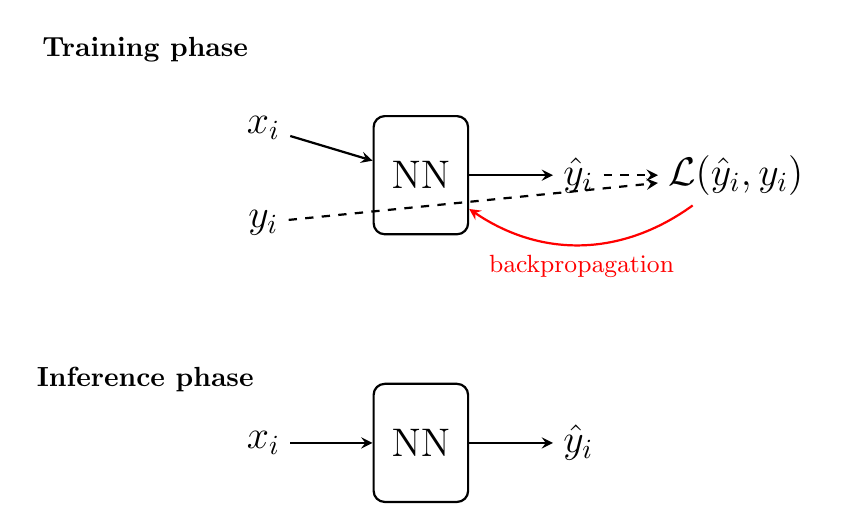
\begin{tikzpicture}[>=stealth, thick, node distance=1.8cm]
        % Training phase
        \node at (-1.5, 2) {\textbf{Training phase}};
        \node (xtrain) at (0,1) {\Large $x_i$};
        \node (ytrain) at (0,-0.2) {\Large $y_i$};
        \node[draw, rounded corners, minimum width=1.2cm, minimum height=1.5cm] (nntrain) at (2,0.4) {\Large NN};
        \node (yhattrain) at (4,0.4) {\Large $\hat{y}_i$};
        \node (loss) at (6,0.4) {\Large $\mathcal{L}(\hat{y}_i, y_i)$};

        % Training arrows
        \draw[->] (xtrain) -- (nntrain);
        \draw[->] (nntrain) -- (yhattrain);
        \draw[->, dashed] (ytrain) -- (loss);
        \draw[->, dashed] (yhattrain) -- (loss);
        \draw[->, thick, red] (loss) to[bend left=35] node[midway, below] {\small backpropagation} (nntrain);
        % Inference phase
        \node at (-1.5, -2.2) {\textbf{Inference phase}};
        \node (xtest) at (0,-3) {\Large $x_i$};
        \node[draw, rounded corners, minimum width=1.2cm, minimum height=1.5cm] (nntest) at (2,-3) {\Large NN};
        \node (yhattest) at (4,-3) {\Large $\hat{y}_i$};
        % Inference arrow
        \draw[->] (xtest) -- (nntest);
        \draw[->] (nntest) -- (yhattest);

    \end{tikzpicture}
    \caption{Illustration of neural network training and inference. During training, both input-output pairs \((x_i, y_i)\) are provided to compute the loss \(\mathcal{L}(\hat{y}_i, y_i)\) and update model parameters via backpropagation. During inference, only the input \(x_i\) is given, and the trained network produces an estimated output \(\hat{y}_i\).}
    \label{fig:nn-train-infer}
\end{figure}

Similarly to supervised learning algorithms, a neural network assumes a data input and constructs an output, based on a collection of data instances, in order to find a suitable representation between them, via a process called \textit{training}. By processing such ground truth input and output pairs, training the model employs a \textit{supervised learning scheme} (see Figure \ref{fig:nn-train-infer}). In practice, training the model refers to adjusting its set of trainable parameters (such as the weight between neurons as illustrated before) in order to find the relationship between the input and target data pairs (assuming it exists). Training such a model consists of numerous important steps. As training consists of a mathematical optimization approach (since the problem is intractable), the goal is to minimize an objective function (loss function) that measures the error in performance, often as the absolute difference between the model's estimated outputs and the ground truth targets. Minimization of such a function is attained by the adjustment of the trainable parameters, which occurs iteratively as dictated by the training \textit{optimizer}, based on gradients computed through \textit{backpropagation} \citep{lecun1988theoretical, werbos2002backpropagation}. Backpropagation applies the chain rule of calculus in reverse (illustrated in Figure \ref{fig:building-blocks}), computing how much each parameter contributed to the error signal. This allows the optimizer to make informed adjustments. Common optimizers include Stochastic Gradient Descent (SGD) \citep{ruder2016overview} and Adam \citep{kingma2015adam}, both of which aim to efficiently navigate the high-dimensional loss landscape.

Once trained, the model can generalize to unseen data in the \textit{inference phase}, where it takes only input \(x_i\) and outputs a prediction \(\hat{y}_i\). Neural network models are known as universal approximators \citep{hornik1989multilayer}. This illustrates that in cases where statistical, machine learning, or even very simple methods fail due to the intractable nature of the function \(f\) between input and output, it becomes significant to consider fitting a neural network model.

Progress in neural networks and deep learning has often been driven by the development of general-purpose architectures that outperform prior methods across a wide range of tasks. Some advancements stem from novel ideas that reshape the field, while others result from the resurgence of older techniques enabled by increased data availability and computational power. Early models such as perceptrons \citep{rosenblatt1958perceptron} laid the foundation for modern neural networks, but their inability to represent non-linearly separable functions, such as XOR \citep{minsky1969perceptrons}, led to skepticism and a temporary stagnation in research. During the 1980s and 1990s, more expressive models were proposed, including self-organizing maps (SOMs) \citep{kohonen1982self}, Hopfield networks \citep{hopfield1982neural} and Boltzmann machines \citep{ackley1985learning}, all of which introduced new paradigms in unsupervised learning, associative memory and energy-based modeling. With the resurgence of deep learning, driven by larger datasets and modern hardware, architectures like feedforward networks, convolutional neural networks (CNNs) \citep{lecun1989backpropagation}, recurrent neural networks (RNNs) \citep{rumelhart1986learning} and LSTMs \citep{hochreiter1997long} became dominant in practical applications. Meanwhile, methods such as support vector machines (SVMs) \citep{cortes1995support} and conditional random fields (CRFs) \citep{lafferty2001conditional} contributed significantly to structured prediction tasks before deep learning approaches took center stage. A key turning point came with the introduction of Transformers \citep{vaswani2017attention}, which moved beyond the limitations of recurrence-based models by relying entirely on attention mechanisms. This shift enabled greater parallelism and improved the ability to capture long-range dependencies, particularly in sequential and structured data. Transformers have since become the backbone of modern foundation models, which aim to generalize across diverse tasks by leveraging vast amounts of data, compute, and expressive representations, an idea that also underpins the work proposed in this thesis.

A neural network consists of multiple \textit{layers}, which may be of the same kind or of different kind, the combination of which can be selected in almost any desired order. A \textit{sequential} architecture consists of layers that are linearly stacked, that is, each layer receives input from only its previous layers and only outputs to its forward layers. The first layer is usually referred to as the \textit{input} layer and the last one as the \textit{output} layer, with the in-between layers referred as \textit{hidden layers} (unscreen blocks). In a way, such a neural architecture can be thought as a stack of building blocks, each of which is responsible for a specific task, from bottom to top (Figure \ref{fig:building-blocks}). All layers consist of different number of parameters (real numbers, vectors or matrices) based on their design. The parameters that are tunable during training are called \textit{trainable} or \textit{learnable parameters}. The collection \(\theta\) of trainable parameters represent the neural network \(f_\theta\). Typically those are the weights (noted by \(W\), \(w\), or \(U\), \(u\)) and biases (notated \(b\)). Depending on the layer's defined operation, these weights are applied to its input \(x\), and by adding the biases \(b\), one obtains its resulting output \(y\). This output will then be fed as input into the next layer and so forth, until the output layer delivers the final estimation of the model. Layers that do not introduce any trainable parameters exist, such as ones that apply operations (e.g. averaging, pooling etc.). They are usually added in order to prepare the data from the previous layer to be fed to the upcoming layers. They may also be applied by taking the network's final output layer and formulating the final predictions of the overall model.

\begin{figure}[ht!]
    \centering
    \begin{tikzpicture}
        % Draw the module
        \draw[thick] (-2, 1) rectangle (2, -1);
        \node at (0, 0) {$f$};
        
        % Input x
        \draw[->, thick, green!50!black] (-3, 0) -- (-2, 0);
        \node[above, green!50!black] at (-2.5, 0) {$x$};
        
        % Output y
        \draw[->, thick, green!50!black] (2, 0) -- (4, 0);
        \node[above, green!50!black] at (2.5, 0) {$y$};
        
        % Gradients
        \draw[<-, thick, red] (-3, -0.5) -- (-2, -0.5);
        \node[below, red] at (-2.5, -0.5) {$\frac{\partial E}{\partial x}$};
        
        \draw[<-, thick, red] (3, -0.5) -- (2, -0.5);
        \node[below, red] at (2.5, -0.5) {$\frac{\partial E}{\partial y}$};
        
        \node[red] at (0, -0.8) {$\frac{\partial y}{\partial x}$};
        
        % Chain rule
        \node[red] at (-2.5, -1.5) {$\frac{\partial E}{\partial x} = \frac{\partial E}{\partial y} \cdot \frac{\partial y}{\partial x}$};

        % Lego placeholder
        \node at (7, 0) {\includegraphics[width=5cm]{images/figures/building_blocks.jpg}};
    \end{tikzpicture}
    \caption{Training deep neural networks can be thought as building blocks, leaving architecture and capabilities to the imagination, with gradients being computed during backpropagation.} \label{fig:building-blocks}
\end{figure}

Apart from selecting the architecture of the model, consisting of the type, amount and order of layers, there are other types of parameters to choose from within each specific layer. Such are called \textit{hyperparameters} such as weight initializers, stride, dilation rate, padding etc. In order to successfully train a network, optimal selection of layers, parameters and hyperparameters, as well as their initialization, are all crucially important. Overall, assembling a neural network model after defining the problem at hand is a non-trivial and demanding task. It requires familiarity with the specific problem, creativity, competence and knowledge within the area of neural networks, plus being informed about the latest advancements and state-of-the-art approaches. It should be noted that selection of the ideal architecture and parameters is a different field at first place, as inevitably to this day it still requires careful fiddling, guessing, experimental trial-and-error procedures and at many times ad-hoc approaches that are empirically shown to improve the state-of-the-art. Finally, although simple in theory, training deep models in practice presents challenges such as vanishing gradients, overfitting, and instability. Techniques like normalization layers, residual connections, and regularization help mitigate these issues. A discussion on how some of the above issues are mitigated is presented in Chapter \ref{chap:training}.